\documentclass{article}
\usepackage{tikz, comment}
\usepackage{pifont}
\usepackage{fontspec, pgfplots}
\usetikzlibrary{arrows, decorations.markings, decorations.pathreplacing}
\begin{comment}
:Title: Not defined yet
:Tags: aa similarity;aas congruence, saa congruence ;abscissa;absolute convergence, absolutely convergent ;absolute maximum, absolute max, global maximum, global max
:Prob: nan;nan;nan;nan;nan
:Author: Prof.Hu Ji-shan, HKUST
:Slug: No name yet

Description Here.........
\end{comment}
\begin{document}\centering

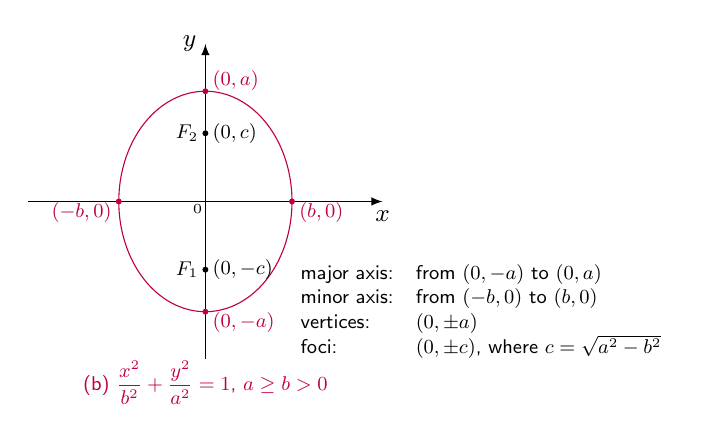
\begin{tikzpicture}[>=latex,xscale=.5*1, yscale=.5*1][font=\sf\small] 

\draw[->] (-4.5, 0) -- (4.5, 0)node[below] {\small $x$};
\draw[->] (0, -4) -- (0, 4)node[left] {\small $y$};

\node[purple, scale=0.8] at (0, -4.6) {(b) $\displaystyle \frac{x^2}{b^2}+\frac{y^2}{a^2}=1$, $a \ge b > 0$};

\node[scale=0.8] at (7, -2.8) {$
\begin{array}{ll}
\hbox{major axis:} &\hbox{from $(0, -a)$ to $(0, a)$}\\
\hbox{minor axis:} &\hbox{from $(-b, 0)$ to $(b, 0)$}\\
\hbox{vertices:} & (0, \pm a) \\
\hbox{foci:} & \hbox{$(0, \pm c)$, where $c = \sqrt{a^2-b^2}$} 
\end{array}
$};

\draw[purple, samples=100, smooth, domain=0:2*pi, variable=\t]
		plot ({2.2*sin(\t r)}, {2.8*cos(\t r)}) ;

\draw[fill] (0, {-sqrt(2.8^2-2.2^2)}) circle(0.06) node[left, scale=0.8]{$F_1$} node[right, scale=0.8]{$(0, -c)$} ;
\draw[fill] (0, { sqrt(2.8^2-2.2^2)}) circle(0.06) node[left, scale=0.8]{$F_2$} node[right, scale=0.8]{$(0,  c)$} ;

\draw[purple, fill] (0, -2.8) circle(0.06) node[right, yshift=-4, scale=0.8]{$(0,-a)$};
\draw[purple, fill] (0,  2.8) circle(0.06) node[right, yshift=4, scale=0.8]{$(0, a)$};

\draw[purple, fill] (-2.2, 0) circle(0.06) node[left, yshift=-4, scale=0.8]{$(-b, 0)$};
\draw[purple, fill] ( 2.2, 0) circle(0.06) node[right, yshift=-4, scale=0.8]{$(b, 0)$};

\node at (-0.2/1, -0.2/1) {\tiny$0$};

\end{tikzpicture}
\end{document}